% Generated by Listas/make_statements.py from pratica-lecture-03.md, item 5. Do not edit.
\textbf{Source.} Muñoz-Garcia \& Toro-Gonzalez (2019), \emph{Strategy and Game Theory: Practice Exercises with Answers}, Ch. 4, Exercise 4 ``Sequential Version of the Battle of the Sexes Game'', p.~163 {[}PDF 175{]}. Reproduced verbatim (statement only; the book's worked answer follows it). \emph{Note (not in the book):} part (a) as printed swaps the roles; the wife moves first, so read it as the husband's best responses to each of the wife's actions, which is what the book's answer computes.



\begin{quote}

Consider the game tree in Fig. 4.13, representing the sequential-move version of the Battle of the Sexes game, where wife acts first, and observing its move husband responds.



\pandocbounded{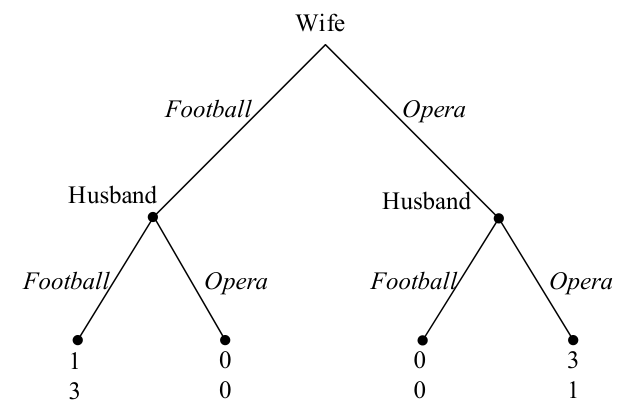
\includegraphics[keepaspectratio,alt={Fig. 4.13 Battle of the sexes sequential-move game}]{../figures/munoz-garcia-4-4.png}}



\emph{Fig. 4.13} Battle of the sexes sequential-move game



\begin{enumerate}

\def\labelenumi{(\alph{enumi})}

\item

  Find the best responses of the wife, for each of the husband's actions.

\item

  Find the husband's equilibrium action and describe the subgame perfect Nash equilibrium of the game.

\item

  Does the equilibrium behavior in the sequential-move game differ from its simultaneous-move version?

\end{enumerate}

\end{quote}

